\section{RTC::Mode\-Capable Interface Reference}
\label{interfaceRTC_1_1ModeCapable}\index{RTC::ModeCapable@{RTC::ModeCapable}}
Execution\-Semantics::Mode\-Capable interface.  


{\tt import \char`\"{}RTC.idl\char`\"{};}

Inheritance diagram for RTC::Mode\-Capable::\begin{figure}[H]
\begin{center}
\leavevmode
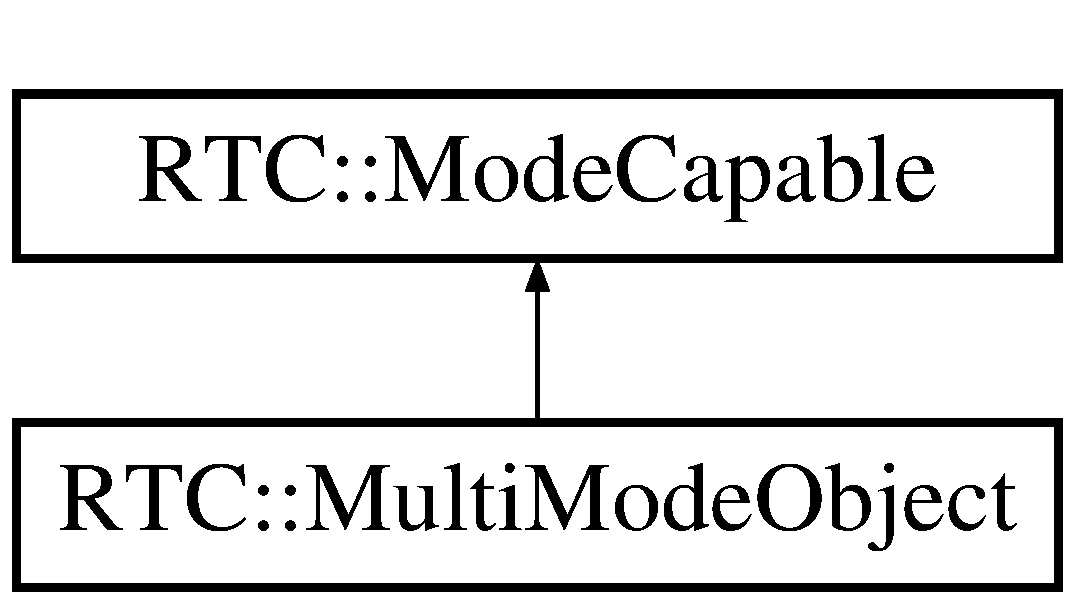
\includegraphics[height=2cm]{interfaceRTC_1_1ModeCapable}
\end{center}
\end{figure}
\subsection*{Public Member Functions}
\begin{CompactItemize}
\item 
{\bf Mode} {\bf get\_\-default\_\-mode} ()
\item 
{\bf Mode} {\bf get\_\-current\_\-mode} ()
\item 
{\bf Mode} {\bf get\_\-current\_\-mode\_\-in\_\-context} (in {\bf Unique\-Id} ec\_\-id)
\item 
{\bf Mode} {\bf get\_\-pending\_\-mode} ()
\item 
{\bf Mode} {\bf get\_\-pending\_\-mode\_\-in\_\-context} (in {\bf Unique\-Id} ec\_\-id)
\item 
{\bf Return\-Code\_\-t} {\bf set\_\-mode} (in {\bf Mode} new\_\-mode, in boolean immediate)
\end{CompactItemize}


\subsection{Detailed Description}
Execution\-Semantics::Mode\-Capable interface. 



\subsection{Member Function Documentation}
\index{RTC::ModeCapable@{RTC::Mode\-Capable}!get_current_mode@{get\_\-current\_\-mode}}
\index{get_current_mode@{get\_\-current\_\-mode}!RTC::ModeCapable@{RTC::Mode\-Capable}}
\subsubsection{\setlength{\rightskip}{0pt plus 5cm}{\bf Mode} RTC::Mode\-Capable::get\_\-current\_\-mode ()}\label{interfaceRTC_1_1ModeCapable_RTC_1_1MultiModeObjecta1}


\index{RTC::ModeCapable@{RTC::Mode\-Capable}!get_current_mode_in_context@{get\_\-current\_\-mode\_\-in\_\-context}}
\index{get_current_mode_in_context@{get\_\-current\_\-mode\_\-in\_\-context}!RTC::ModeCapable@{RTC::Mode\-Capable}}
\subsubsection{\setlength{\rightskip}{0pt plus 5cm}{\bf Mode} RTC::Mode\-Capable::get\_\-current\_\-mode\_\-in\_\-context (in {\bf Unique\-Id} {\em ec\_\-id})}\label{interfaceRTC_1_1ModeCapable_RTC_1_1MultiModeObjecta2}


\index{RTC::ModeCapable@{RTC::Mode\-Capable}!get_default_mode@{get\_\-default\_\-mode}}
\index{get_default_mode@{get\_\-default\_\-mode}!RTC::ModeCapable@{RTC::Mode\-Capable}}
\subsubsection{\setlength{\rightskip}{0pt plus 5cm}{\bf Mode} RTC::Mode\-Capable::get\_\-default\_\-mode ()}\label{interfaceRTC_1_1ModeCapable_RTC_1_1MultiModeObjecta0}


\index{RTC::ModeCapable@{RTC::Mode\-Capable}!get_pending_mode@{get\_\-pending\_\-mode}}
\index{get_pending_mode@{get\_\-pending\_\-mode}!RTC::ModeCapable@{RTC::Mode\-Capable}}
\subsubsection{\setlength{\rightskip}{0pt plus 5cm}{\bf Mode} RTC::Mode\-Capable::get\_\-pending\_\-mode ()}\label{interfaceRTC_1_1ModeCapable_RTC_1_1MultiModeObjecta3}


\index{RTC::ModeCapable@{RTC::Mode\-Capable}!get_pending_mode_in_context@{get\_\-pending\_\-mode\_\-in\_\-context}}
\index{get_pending_mode_in_context@{get\_\-pending\_\-mode\_\-in\_\-context}!RTC::ModeCapable@{RTC::Mode\-Capable}}
\subsubsection{\setlength{\rightskip}{0pt plus 5cm}{\bf Mode} RTC::Mode\-Capable::get\_\-pending\_\-mode\_\-in\_\-context (in {\bf Unique\-Id} {\em ec\_\-id})}\label{interfaceRTC_1_1ModeCapable_RTC_1_1MultiModeObjecta4}


\index{RTC::ModeCapable@{RTC::Mode\-Capable}!set_mode@{set\_\-mode}}
\index{set_mode@{set\_\-mode}!RTC::ModeCapable@{RTC::Mode\-Capable}}
\subsubsection{\setlength{\rightskip}{0pt plus 5cm}{\bf Return\-Code\_\-t} RTC::Mode\-Capable::set\_\-mode (in {\bf Mode} {\em new\_\-mode}, in boolean {\em immediate})}\label{interfaceRTC_1_1ModeCapable_RTC_1_1MultiModeObjecta5}




The documentation for this interface was generated from the following file:\begin{CompactItemize}
\item 
{\bf RTC.idl}\end{CompactItemize}
